%%%%%%%%%%%%%%%%%%%%%%%%%%%%%%%%%%%%%%%%%%%%%%%%%%%%%%%%%%%%%%%%%%%%
\section{Production and Assembly} % (8 pages)}
\label{sec:fdsp-apa-prod-assy}

Design, construction, and testing of the DUNE Far Detector APAs is overseen by the DUNE APA Consortium within the Collaboration.  The APA Consortium will take a ``factory style'' approach to the construction with multiple factories being planned in the US and UK. This approach will allow the consortium to produce APAs at the rate required to meet overall construction milestones and at the same time reduce risk to the project if any location encounters problems that slow the pace of production.

%%%%%%%%%%%%%%%%%%%%%%%%%%%%%%%%%%%
%\subsection{APA Production Plan}
%\label{sec:fdsp-apa-prod-plan}

The starting point for the APA production plan for the DUNE Far Detectors is the experience and lessons learned from ProtoDUNE construction. For ProtoDUNE, APAs have been constructed both at the Physics Sciences Laboratory (PSL) at the University of Wisconsin and at Daresbury Laboratory in the UK.  APA construction for DUNE is also envisaged to be done at US and UK collaborating institutions, however, assuming construction begins in 2021, a minimum of 6 production lines is required to build 150 APAs within 2.5 years for the first DUNE \SI{10}{kton} module.   

Based on the ProtoDUNE experience, we estimate that each APA will require approximately 50 shifts (8 hour intervals) of effort to construct. This begins with installation of the APA frame into the winding machine and assumes that all hardware necessary for construction is ready to go at the factory. Currently an APA can be built in 64 shifts. Several improvements to the process and tooling are planned that will bring this down to the required 50 shifts. The production model assumes that factories will run two shifts per day and that 2 weeks per year are devoted to maintenance of equipment. 

Each production line is centered around a wire winding robot, or ``winder'', that makes the continuous wrapping of wire on a \SI{6}{m} long frame possible. The winder can also be used to make wire tension measurements by replacing the winding head with a laser photo diode system that then can determine an individual wire's natural frequency and hence its tension. A production line also requires two ``process carts''. These carts support the APA and are used during various steps in the construction process, e.g. continuity testing, board epoxy installation, etc. A production line, therefore, requires a means of lifting the APA in and out of the winder. A gantry-style crane has been used for ProtoDUNE construction.

%%%%%%%%%%%%%%%%%%%%%%%%%%%%%%%%%%%
\subsection{Facility Plans}
\label{sec:fdsp-apa-facility}

Construction of DUNE Far Detector APAs will take place in both the US and the UK. Daresbury Lab in the UK will house multiple production lines, one of which already exists from ProtoDUNE. In the US, it's anticipated that production lines will be set up at the University of Chicago, Yale University, and the already existing production facility at the University of Wisconsin, PSL. At least eight APA production lines spread over multiple facilities will provide some margin on the production schedule and provide backup in the event that technical problems occur at any particular site. 

The space requirements for each production line are driven by the large size of the APA frames and the winding robot used to build them. The approximate dimensions of the clean space to house winder operations and associated tooling is \SI{175}{m$^2$}. The estimated requirement for inventory, work in progress, and completed APAs is about \SI{600}{m$^2$}. Each facility will also need temporary access to shipping and crating space of about \SI{200}{m$^2$}. Possible floor layouts at each institution are shown in Figure~\ref{fig:factories}. Adequate space is available at each site and commitments have been expressed by each of the institutions for its use on DUNE. 

The University of Wisconsin has space available within the Physical Sciences Lab Rowe Technology Center. A portion of the vault area within PSL's Rowe Technology Center has been setup and has been used for the past two years for the ProtoDUNE project. There is approximately \SI{20,000}{ft$^2$} (\SI{1,850}{m$^2$}) available for DUNE and the possibility exists to expand the current clean tent to house another production line, if needed. 

ProtoDUNE construction has also taken place at Daresbury Lab.  The current facility cannot accommodate multiple production lines, but the ``Inner Hall'' on the Daresbury site has been identified as an area that is sufficiently large to be used for DUNE APA construction. It has good access and crane coverage throughout. Daresbury Laboratory management have agreed that the area is available, but it would need investment to establish a safe working environment. Preparation work for the construction area is underway with a \pounds200k investment to clear the current area of existing facilities, obsolete cranes, and ancillary equipment. Also planned is the renovation of a plant room which will be used for storage and as a shipping area. This work is ongoing. The production factory is being designed to hold 4 winding machines and associated process equipment and tooling. The factory will be available for 2020 when it is planned that production will begin. 

The Enrico Fermi Institute at the University of Chicago and the Wright Laboratory at Yale University have the needed infrastructure to house one or two APA production lines as well. Development work that is relevant for local planning at each site has begun at those institutions.  Figure~\ref{fig:factories} shows conceptual factory layouts at the facilities available on those campuses.

\begin{dunefigure}[Conceptual layouts of APA factories]{fig:factories}
{Possible factory layouts at (clockwise from upper left) PSL, University of Chicago, Daresbury Lab, and Yale University, with two to four winders at each site.}
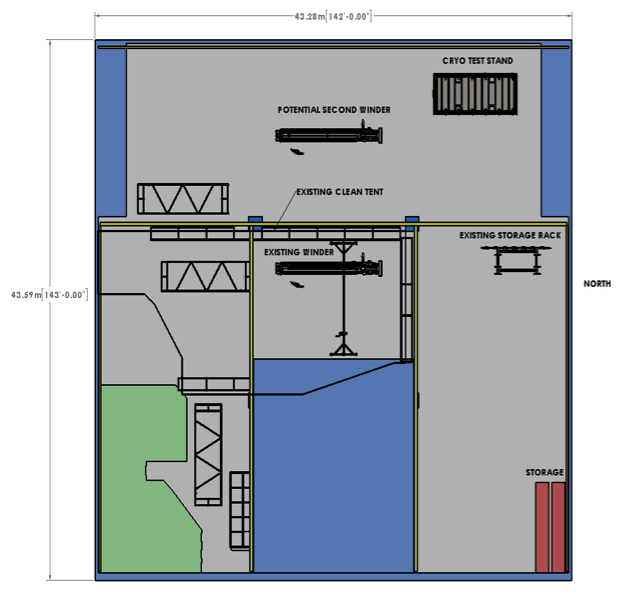
\includegraphics[height=0.28\textheight]{PSL-schematic.png} 
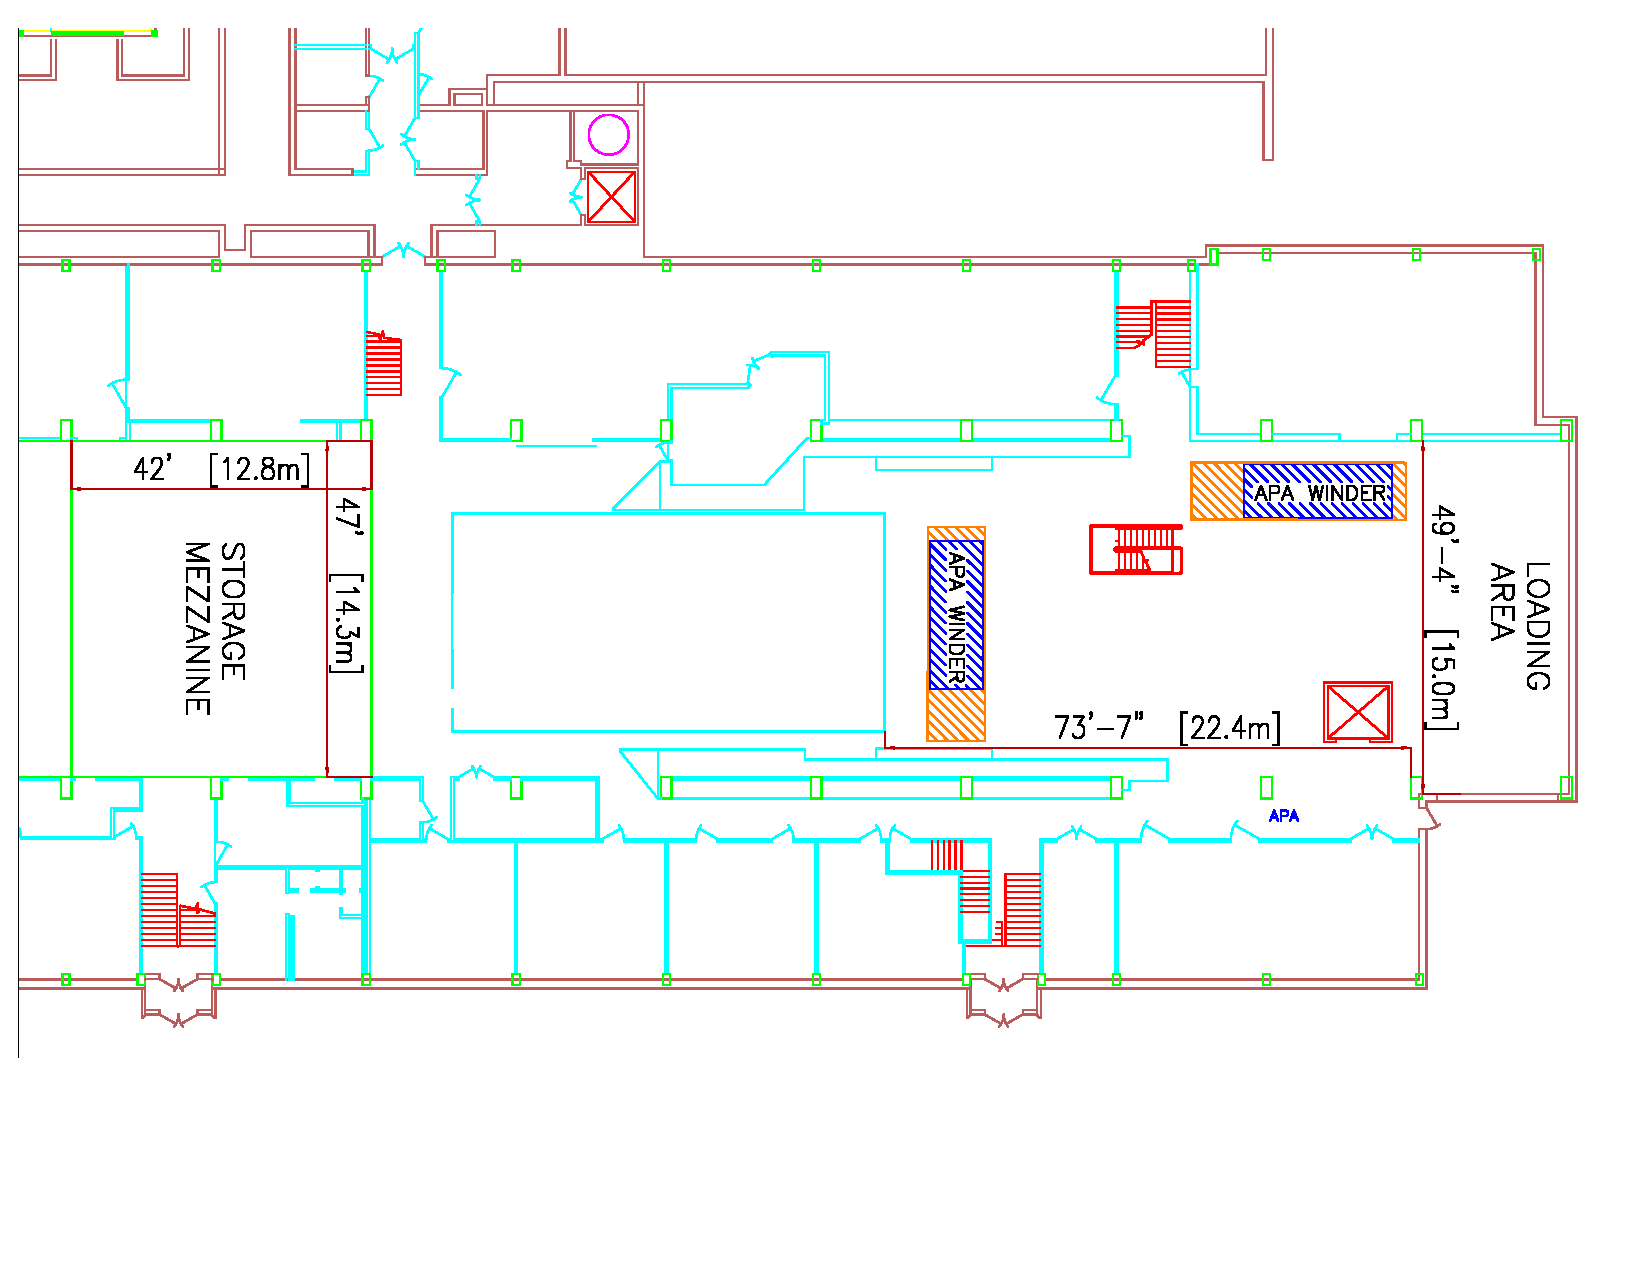
\includegraphics[height=0.26\textheight]{Chicago-2APA.pdf}
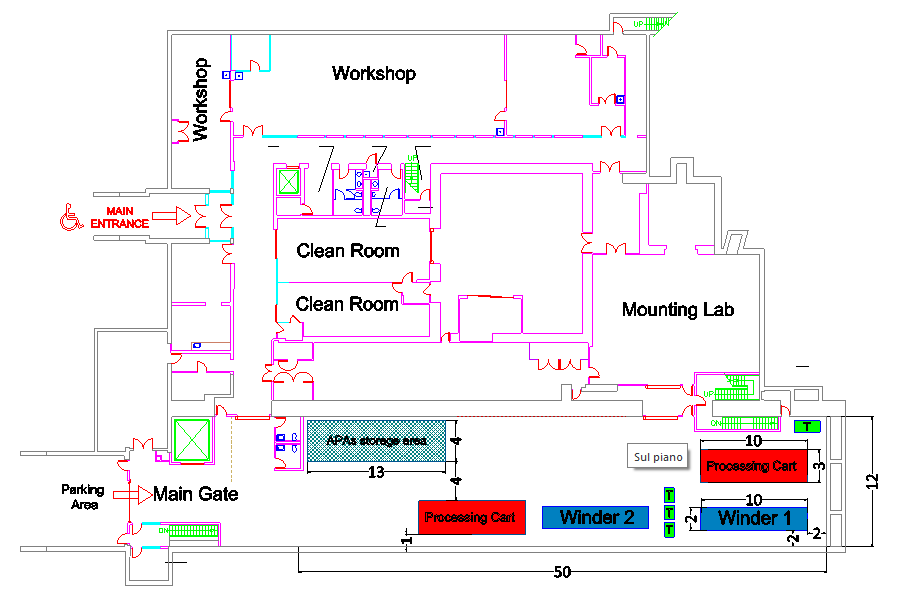
\includegraphics[height=0.27\textheight]{Yale-WL-2APA.png}
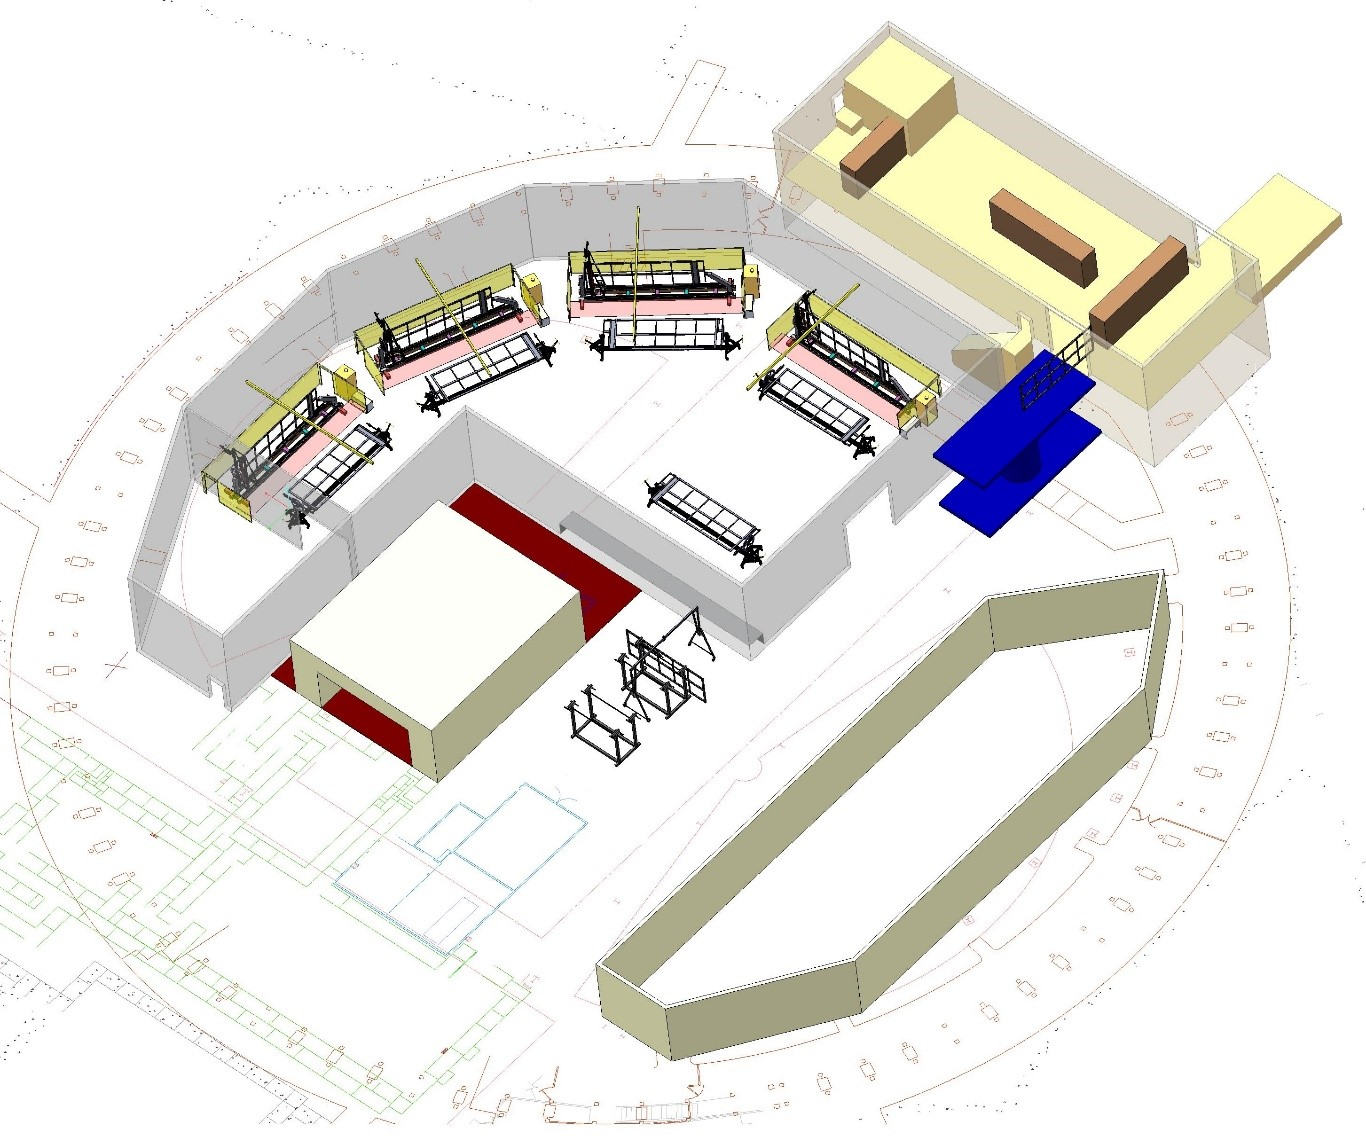
\includegraphics[height=0.27\textheight]{UK-production-factory-layout.jpg} 
\end{dunefigure}


%%%%%%%%%%%%%%%%%%%%%%%%%%%%%%%%%%%
\subsection{Assembly Procedures and Tooling}
\label{sec:fdsp-apa-assy}

A subset of procedures describing how to perform the step-by-step assembly of an APA was originally created prior to the finalization of the ProtoDUNE APA series of drawings, and assigned drawing numbers. During subsequent assemblies, these instructions have evolved due to the addition of better tooling, fixtures, jigs and more complete drawing documents.  The process steps contained in each procedure have also been changed to create a better match with the B.O.M. (Bill Of Materials) contained on each finalized drawing level.  Table~\ref{tab:assembly-docs} lists what documents are available related to each assembly level.  Currently these documents are being revised to reflect the latest evolution of these procedures that were used to assemble US-APA-4 for ProtoDUNE.

\begin{dunetable}[APA assembly documents]{lcc}{tab:assembly-docs}{Procedure documents for APA assembly.}   
APA Assembly Level & \textbf{Drawing No.} & \textbf{Assembly Instructions Doc.} \\ \toprowrule
APA Frame Assembly & 8757 004 & 8752Doc001 \\ 
                   &          & 8752Doc002 \\ \colhline
Comb Base and Mesh & 8757 003 & 8752Doc003 \\
				   &          & 8752Doc004 \\ \colhline
Four Wire Layers   & 8757 002 & ~~~~~8752Doc005 (X) \\
                   &          & ~~~~~8752Doc006 (V) \\
                   &          & ~~~~~8752Doc007 (U) \\
                   &          & ~~~~~8752Doc008 (G) \\ \colhline
Factory APA        & 8757 030 & 8752Doc009 \\
                   &          & 8752Doc010 \\ \colhline
Crating for Shipment & being finalized & being finalized \\
\end{dunetable}

\begin{dunefigure}[Photos of the APA wire winding machine]{fig:winder-photos}{(Left) Partially wired ProtoDUNE APA on the winding machine at Daresbury Lab, UK. (Right) Partially wired ProtoDUNE APA on the winding machine during wire tension measurements at University of Wisconsin, PSL. }
%\vspace*{3ex}
\setlength{\fboxsep}{0pt}
\setlength{\fboxrule}{0.5pt}
\fbox{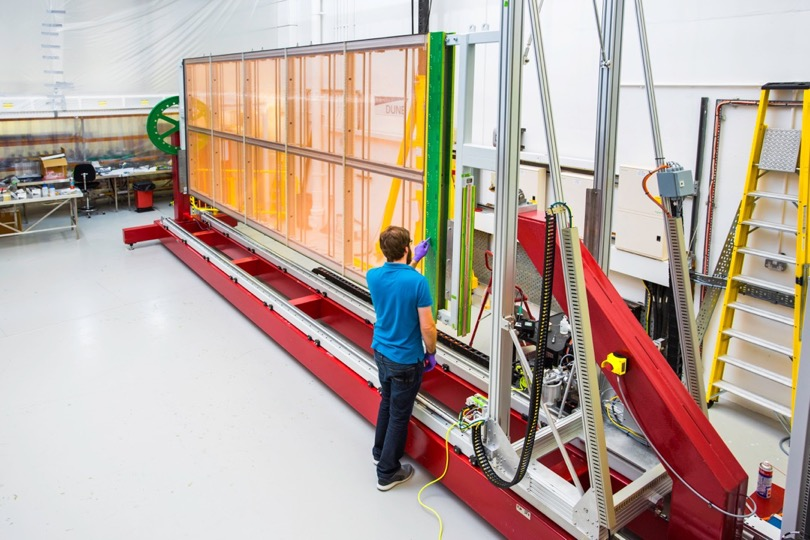
\includegraphics[height=0.3\textheight,trim=25mm 0mm 4mm 0mm,clip]{APAAtDaresbury}}
\fbox{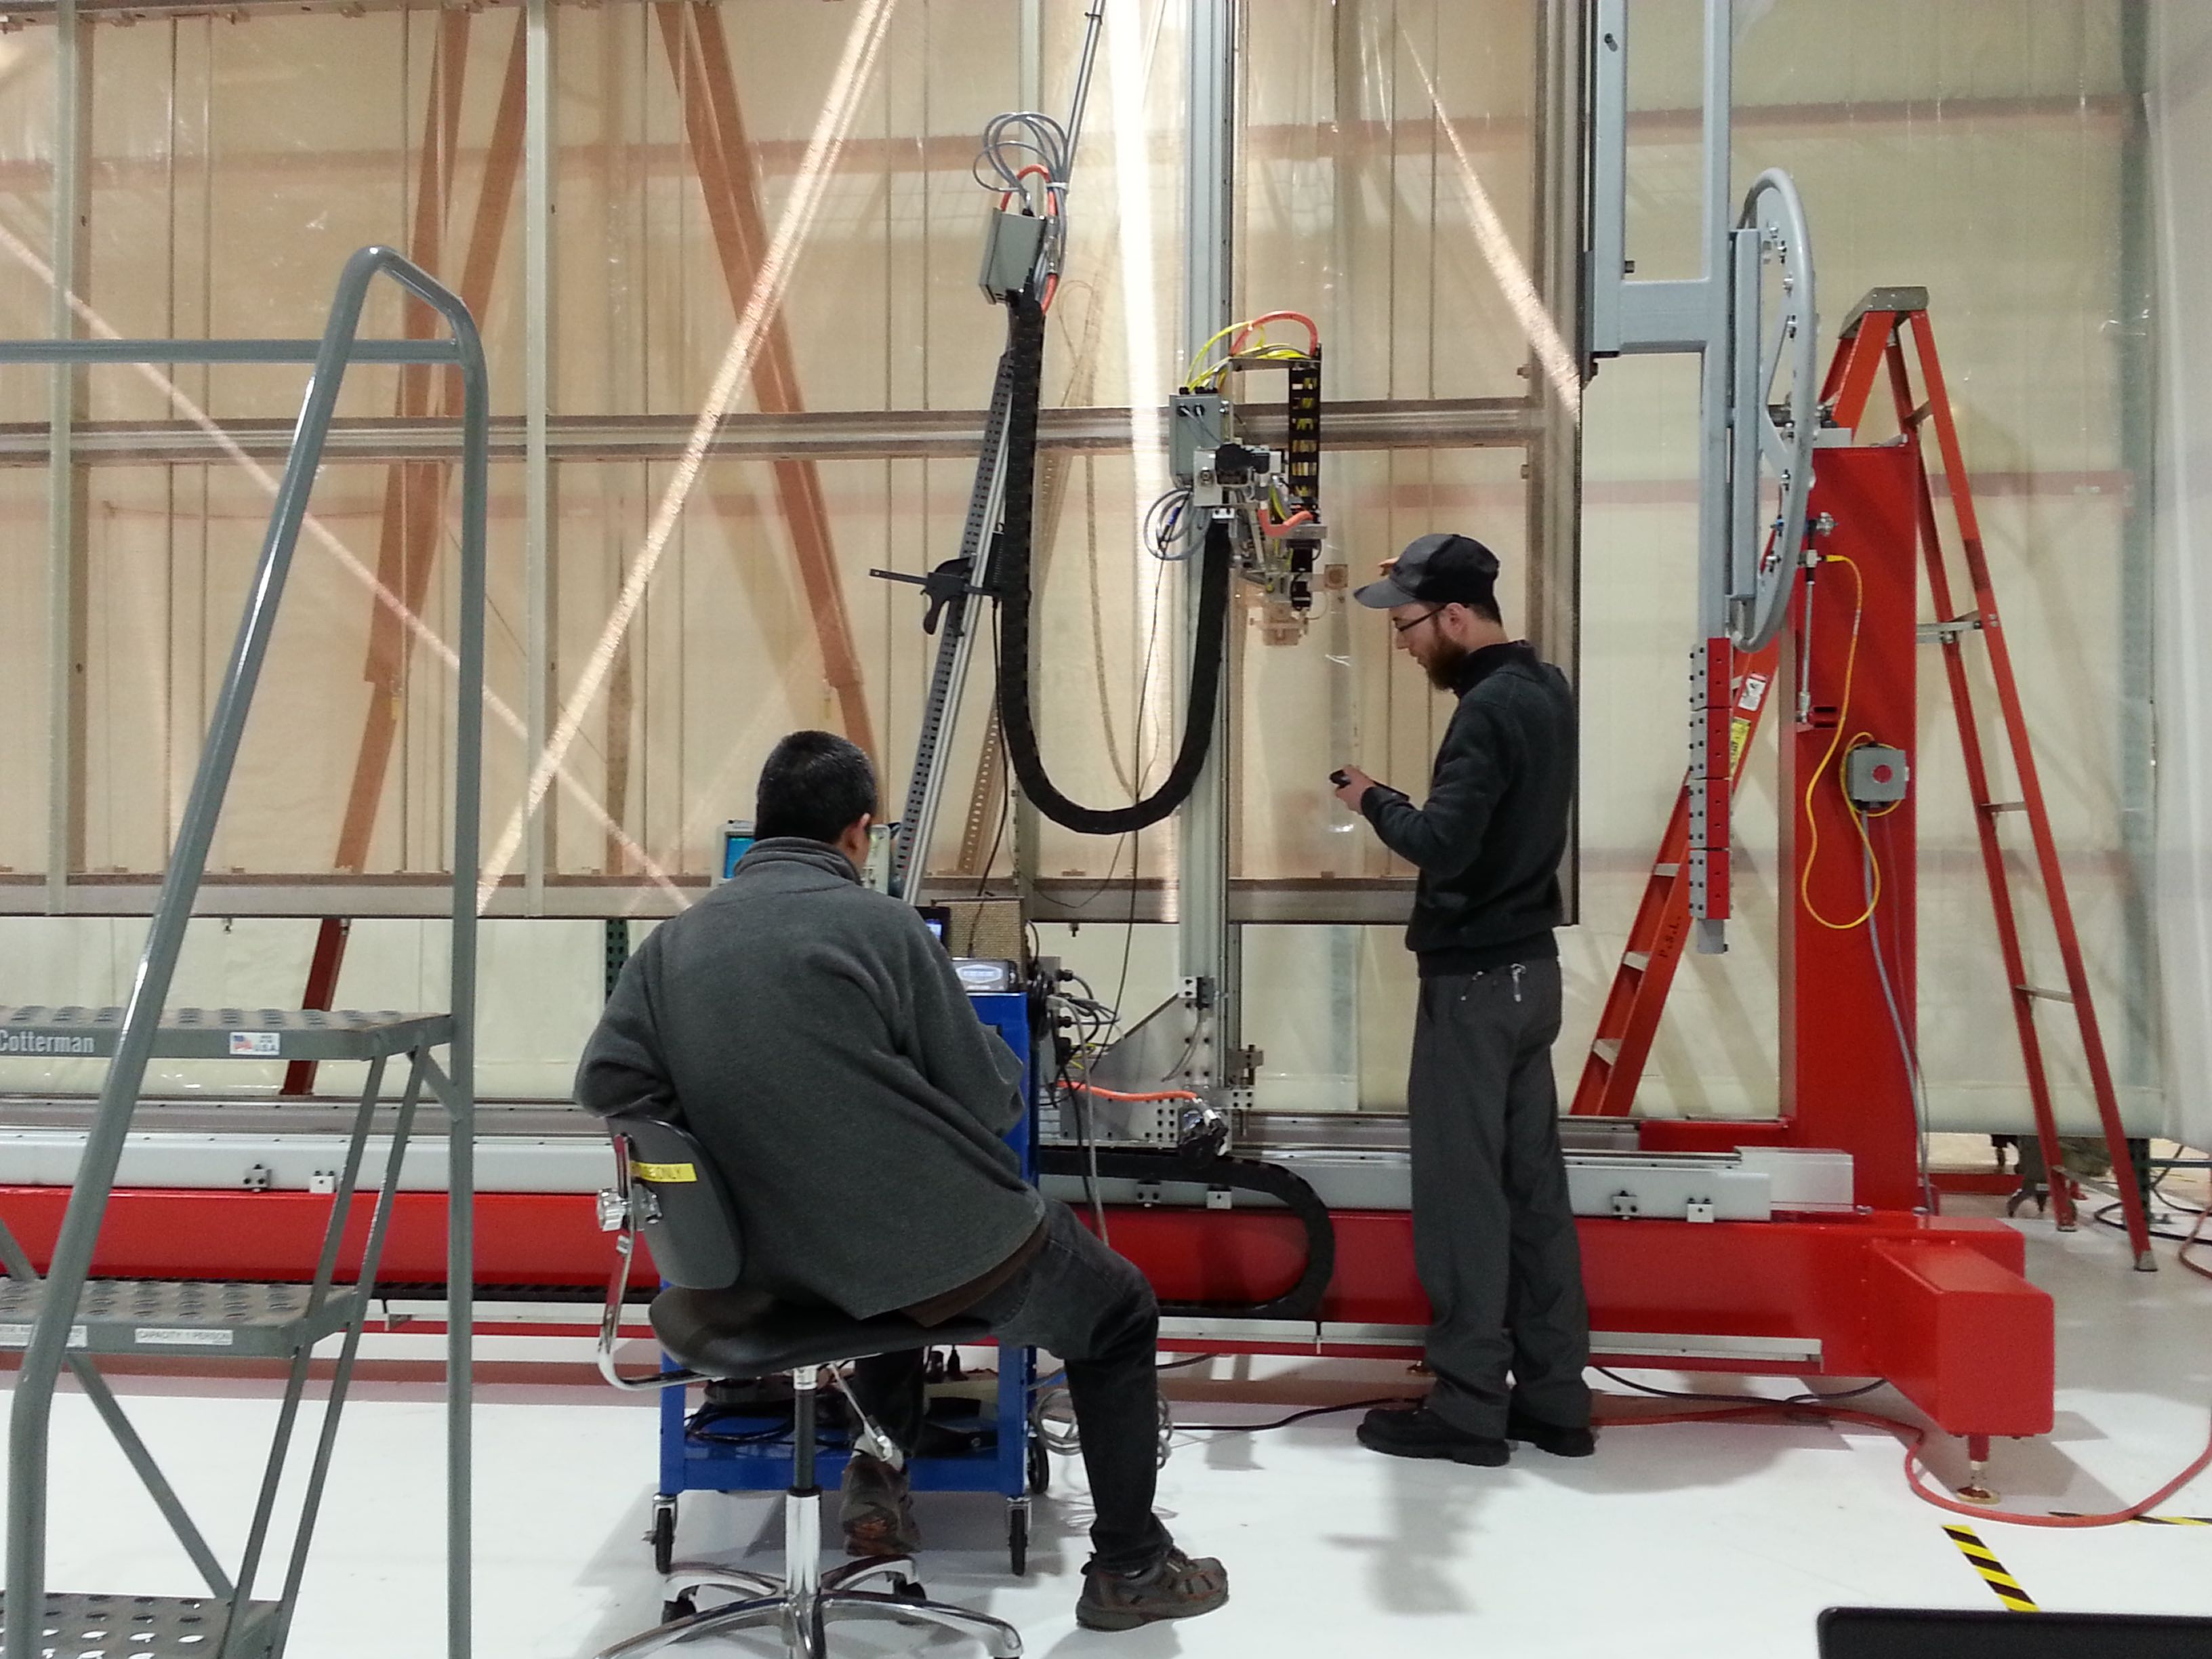
\includegraphics[height=0.3\textheight,trim=200mm 0mm 30mm 0mm,clip]{APA-photo-tension-testing}}
\end{dunefigure}

The central piece of equipment used in APA production is the custom-designed wire winder machine, shown in use in Figure~\ref{fig:winder-photos}.  An important centerpiece of the winder machine is the wiring head.  The head releases wire as motors move it up and down and across the frame, controls the tension in the wire as it gets laid, and positions the wire at solder connection points for soldering by hand. The  fully automated motion of the winder head is controlled by software, which is written in the widely used numerical control G programming language.  The winder also includes a built-in vision system to assist operators during winding, which is currently used at winding start-up to find a locator pin on the wire boards.  During the winding process, an APA moves on and off the winder machine multiple times for wiring, soldering, testing, etc.  

%Current ProtoDUNE APA construction uses a few very large pieces of tooling to facilitate movement and assembly of a bare APA frame and a frame loaded with mesh/boards/wires. 
Two large process carts, as shown in Figure~\ref{fig:apa-process-cart}, are used to move APAs around the assembly facility, and also move them to a shipping/packing location area for loading into specialized crate containers. The process cart with regular casters remains in the assembly area and is maintained at a particular height that coordinates with other construction tooling such as jack stands and platform ladders. A second process cart has been fitted with specialized 360$^\circ$ rotating casters that are instrumental in allowing the process cart loaded with a fully assembled APA to maneuver tight corners during the journey from the assembly area to the shipping/packing location.

\begin{dunefigure}[APA on a process cart]{fig:apa-process-cart}{APA being moved around a production facility on the process cart. Jig for wire comb installation, which is done on the process cart.}
\setlength{\fboxsep}{0pt}
\setlength{\fboxrule}{0.5pt}
\fbox{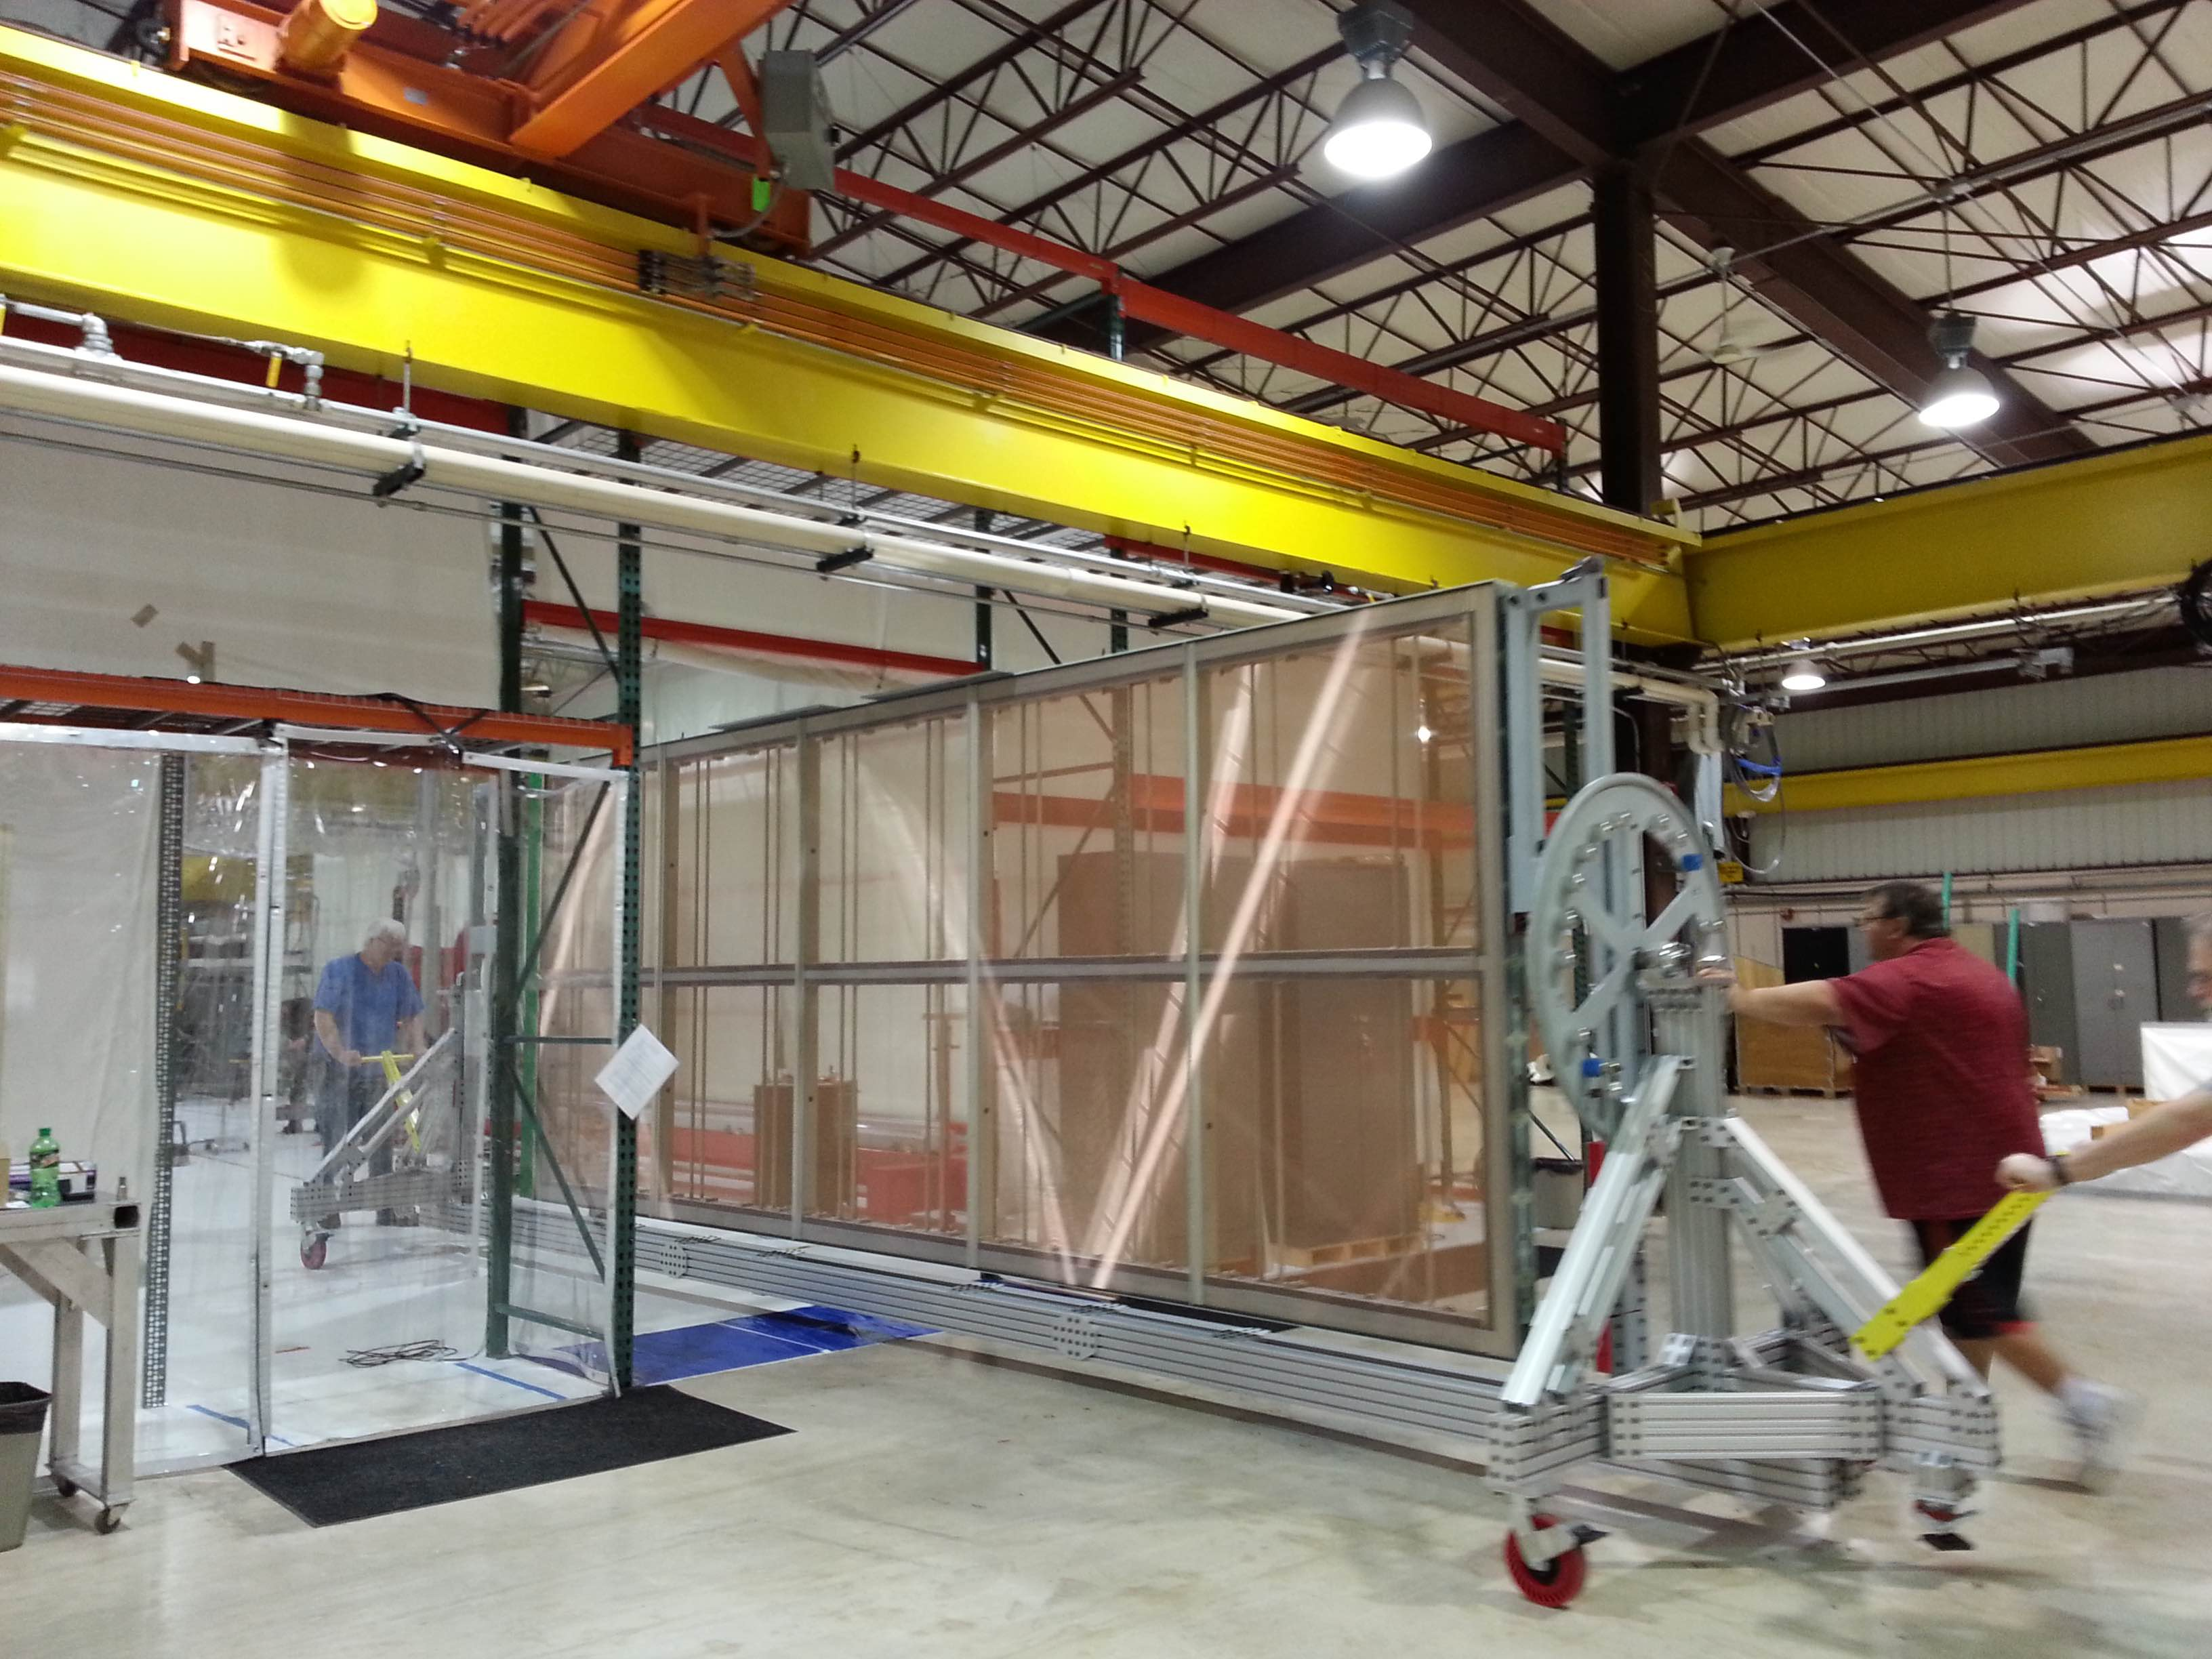
\includegraphics[height=0.24\textheight,trim=50mm 0mm 70mm 0mm,clip]{APA-process-cart.jpg}}
\fbox{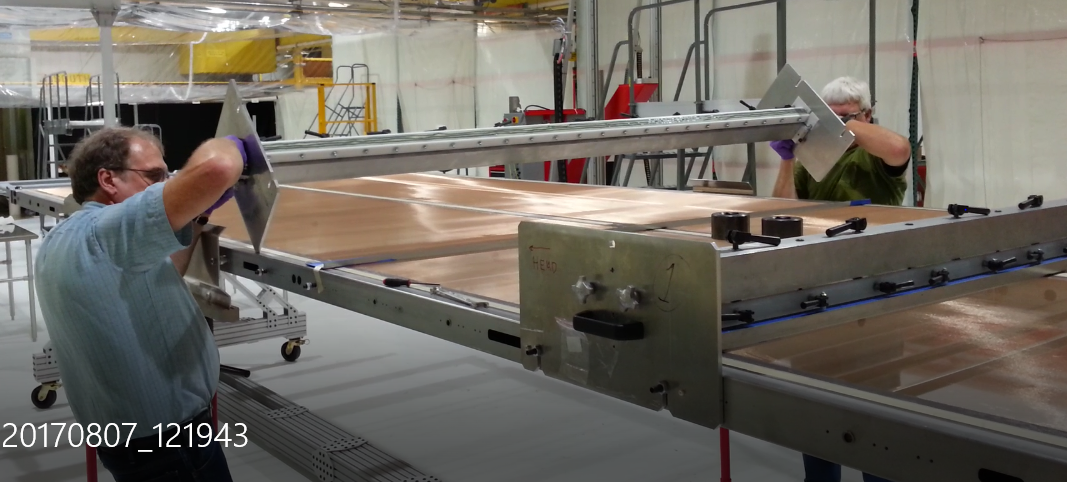
\includegraphics[height=0.24\textheight,trim=15mm 0mm 35mm 0mm,clip]{comb-base-jig.png}}
\end{dunefigure}

%Mesh Attach Jig (and associated Hold-Down Bars)
Before wiring can begin, the first operation with a bare frame is to install the grounding mesh. %This assembly operation is completed by lowering a large mesh attach jig to a frame supported in a horizontal position.  An overhead crane is utilized to lift this large jig while multiple personnel guide it into the appropriate position. 
A large mesh attach jig is needed to hold the mesh in place for gluing. Once the jig is leveled sufficiently to the frame, a mesh panel is laid into place and hold down bars are iteratively moved and repositioned until the mesh is as flat and tight as possible.  The outside edge of the mesh panel then gets epoxied, and the jig and hold down bars remain in place for a 12 hr epoxy cure cycle.  This process is then repeated for the next three shifts until all four panels of mesh have been attached to the bare APA frame.  %When the mesh attach jig is finally dis-engaged from the APA frame, the first level of X foot and head boards are attached with fasteners, and (8) Comb Base assemblies are installed.

%\begin{dunefigure}[APA on a process cart]{fig:apa-process-cart}{APA being moved around a production facility on the process cart.}
%\setlength{\fboxsep}{0pt}
%\setlength{\fboxrule}{0.5pt}
%\fbox{\includegraphics[width=0.5\textwidth]{mesh-stretching.jpg}}
%\fbox{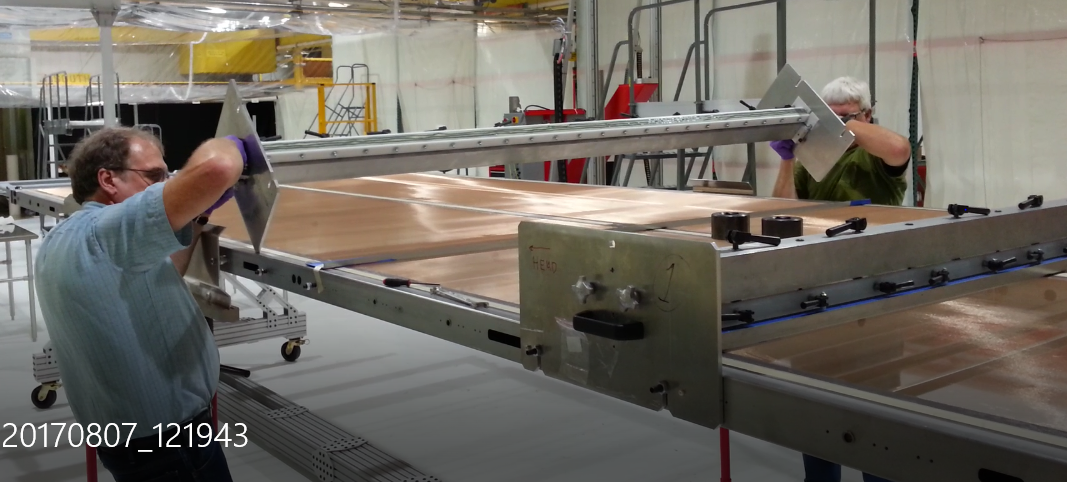
\includegraphics[width=0.5\textwidth]{comb-base-jig.PNG}}
%\end{dunefigure}

%\todo{Pull in a Figure of a Mesh Attach Jig Installation + Mesh panel being held w hold down Bars}


%Comb Base Installation Jig (for X-Layer only)
At the four cross beam locations per each side of the APA, a comb base with $X$-layer combs must be installed above the mesh.  Currently there are two jigs that can be loaded and installed at a time, and after a 6 hr epoxy cure cycle the two jigs are removed from the initial locations and placed in another two locations, on the same side of the APA.  Thus four comb bases are installed within one operation shift and the APA is left in this horizontal position to cure overnight.  The next day, the APA is flipped 180$^\circ$, and the process is repeated for the other side. Figure~\ref{fig:apa-process-cart} shows the comb installation jig in use.  %supported horizontally and two jigs are loaded and installed onto the APA.  A 6 hr epoxy cure cycle is maintained before the (2) jigs are removed, reloaded and installed at the last (2) cross beam locations on the second side of the APA.  The (2) installation jigs are left for an overnight cure in the horizontal position.  

%\todo{Pull in a Figure of the Comb Base Jig Installation + (2) jigs shown attached onto the APA}

%Board Gluing/Epoxying Operations - Various Stencils
%Once the $X$-wire layer has been wound onto the APA and solder joints, tension and electrical testing have been completed, another board layer is installed to cover and protect the first layer of wires.  Board specific stencils are now utilized to control the proper dispensed volume of 2216G epoxy to each different board on the APA that requires epoxy. The process of dispensing, striking and measuring the resulting mass of 2216G is similar for each board type that must receive an epoxied board.  Several matrix documents have been created to ensure the dispensing and installation personnel are using the correct stencil and proper dispensed amount of 2216G to complete these operations.   

%\todo{Pull in a few Figs of stencils/boards + patterns on back of boards}



%%%%%%%%%%%%%%%%%%%%%%%%%%%%%%%%%%%%%%%%%%%%%%%%%%%
\subsection{Material Supply}  

Ensuring the reliable supply of raw materials and parts to each of the factories is critical to keeping APA production on schedule through multiple years of construction. Here the consortium institutions will play a pivotal role taking on the responsibility for the delivery of APA sub-elements to each of the factories. Supplier institutions will have responsibility for the sourcing, inspection, cleaning, testing, quality assurance, and delivery of hardware to each of the factories. 

\begin{itemize}
\item Frame construction: We envision two sources of frames, one in the US and one in the UK. The institutions responsible will rely on many lessons learned from ProtoDUNE. The effort requires specialized resources and skills including a large assembly area, certified welding capability, large scale metrology tools and experience, and large scale tooling and crane support. Two approaches are under consideration for sourcing; one is a total outsource strategy with an industrial supplier, the other is to procure all of the major machined and welded components and then assemble and survey in-house. Material suppliers have been identified and used with good results on ProtoDUNE.
\item Mesh supply and construction: Elsewhere in this proposal we describe the current mesh installation procedure. However, our ProtoDUNE experience leads us to believe that moving to smaller self-supporting ``window screen'' panels will save assembly time and improve overall APA quality. An excellent source of mesh exists and was used on ProtoDUNE.
\item Wire procurement: Wire is a significant element in the assembly of an APA. There is approximately 24 km of wire wound on each unit. Through ProtoDUNE we have worked with an excellent supplier that has worked with us to provide wire that is of high quality and wound on spools that we provide. These spools are then used directly on the winder head with no additional handling or re-spooling required. Wire samples from each spool are strength tested prior to use.
\item Comb procurement: An institution will work with either our existing comb supplier or find additional suppliers that can meet our requirements. The ProtoDUNE supplier has been very reliable.
\item Wire wrapping board procurement: One or more consortium institutions will take on the responsibility of wire wrapping board supply. The side and foot boards are rather unique to suppliers as they have electrical traces and provide wire placement support through a separately bonded tooth strip. There are 276 boards per APA for the X, V, U, G, and covers, or 41,400 needed for 150 APAs. Using costs from ProtoDune, the material cost alone is \$1.8M. The institutions that have responsibility for boards will spend time working with multiple vendors to reduce risk and ensure quality. 
\item Capacitor resistor boards: These boards are rather unique given their thickness, high voltage components, and leakage current requirements. A reliable source of bare boards was found for ProtoDUNE. Assembly and testing was performed at PSL. We will conduct a more exhaustive search of vendors that will be willing to take on assembly and test for the 3000 plus boards needed for DUNE.
\item Winders and tooling: We propose that PSL and Daresbury work together to supply tooling and winding machines for additional production lines at new locations and for additional lines in-house. This is a natural collaboration that has been in place for nearly two years on ProtoDUNE.
\end{itemize}


%%%%%%%%%%%%%%%%%%%%%%%%%%%%%%%%%%%%%%%%%%%%%%%%%%%%%%%%%%%
\subsection{Planned Improvements to Production Process}

Based on our ProtoDUNE experience, we have identified several potential improvements to tooling and process that will allow the APAs to be constructed in a more efficient and reliable manner, including:

\begin{itemize}

\item Wiring head design: Efforts to improve winder head performance are already underway. We envision improved tension control, continuous tension feedback, improved clutch, and an improvement to the compensator mechanism all leading to better, more consistent, and more reliable winder performance.  The current winding head uses a magnetic clutch mechanism that is manually adjusted to increase or decrease the tension of the wire as it is wound around the APA. The clutch regularly needs adjustment as the diameter of the wire on the spool reduces during the winding process. In addition, if the mechanism is run from a `cold start', it has been observed that the tension changes after $\sim$10 minutes of running. Current experience of winding the ProtoDUNE wires shows that it is difficult to maintain the target tension of 5$\pm$\SI{1}{N}.

A solution to this problem is to design a winder head with active tension control. This can be achieved by replacing the magnetic clutch with a servo motor and introducing a potentiometer on a ``dancer arm'' for the feedback loop (see Figure~\ref{fig:winding-head}). This will only work if there are no signal losses when transferring the winding head to the compensator latching mechanism and back. The system can be driven in torque mode and will compensate for any wire spool changes and will be able to operate from a cold start. This development is well underway with tests currently being carried out.

\begin{dunefigure}[Exploded view of the winding machine head]{fig:winding-head}
{Exploded view of winder head with active tension control.}
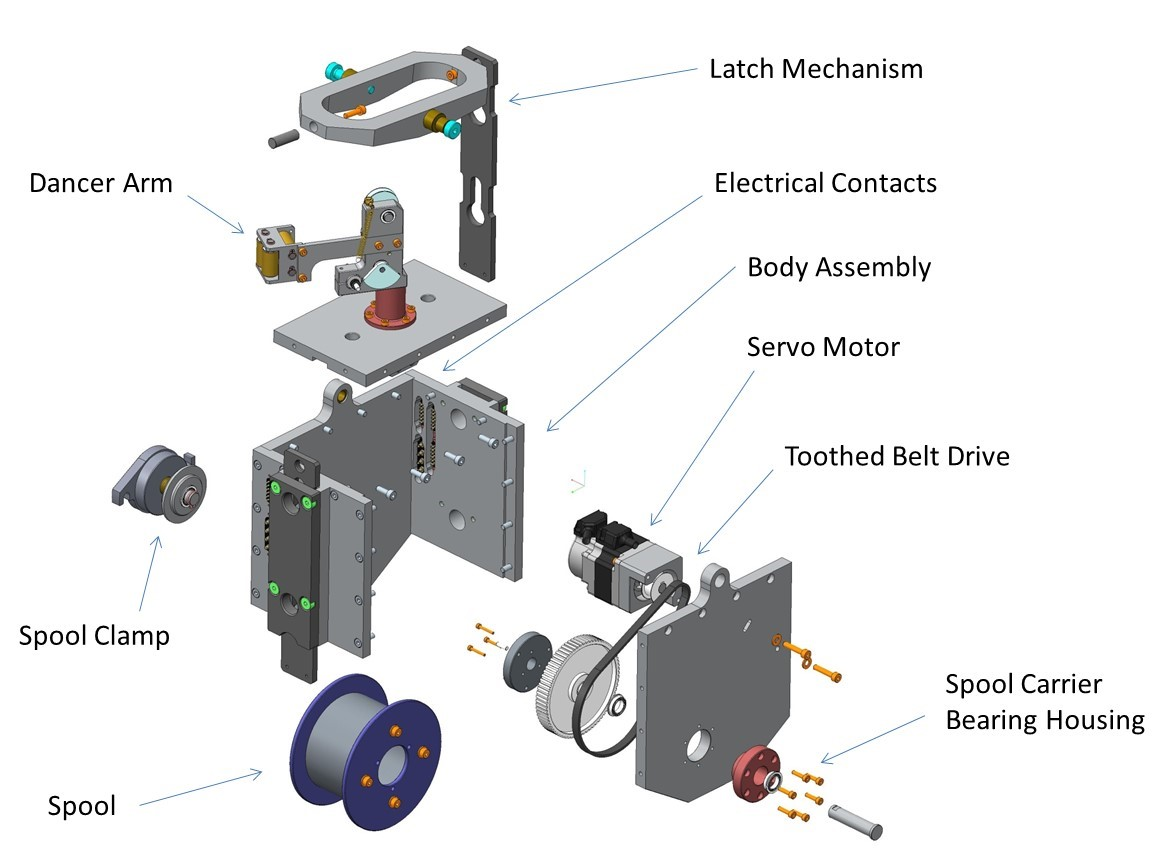
\includegraphics[width=0.7\textwidth]{Winder-head-with-active-tension-controls.jpg}
\end{dunefigure}

\item Winder interface arm design: The current winder interface only allows one-half of a wire plane to be wired at a time. The APA frame must be moved to the process cart where the interface arms are flipped 180$^\circ$ to wind the second half of the wire plane.  A new design concept, illustrated in Figure~\ref{fig:winding-dev}, will allow the winder head to pass from one side to the other in a nearly continuous fashion without removal from the winding machine.  The interface frames are replaced at either end by retractable linear guided shafts. These can be withdrawn to allow passing of the winding head around the frame over the full height of the frame. These shafts have conical ends and locate in shafts that are fixed to the internal frame tube to provide guided location. This design change does not alter the design of the frame. The design also allows for rotation in the winding machine, so that it should also be possible to carry out board installation and gluing \& soldering in the winding machine. This eliminates the need to transfer the APA to the process cart for the whole of the production operation, which is inherently a safer and faster production method as it cuts down the amount of handling of the APA.

\begin{dunefigure}[Winding Machine Dev]{fig:winding-dev}
{Winding machine design development.}
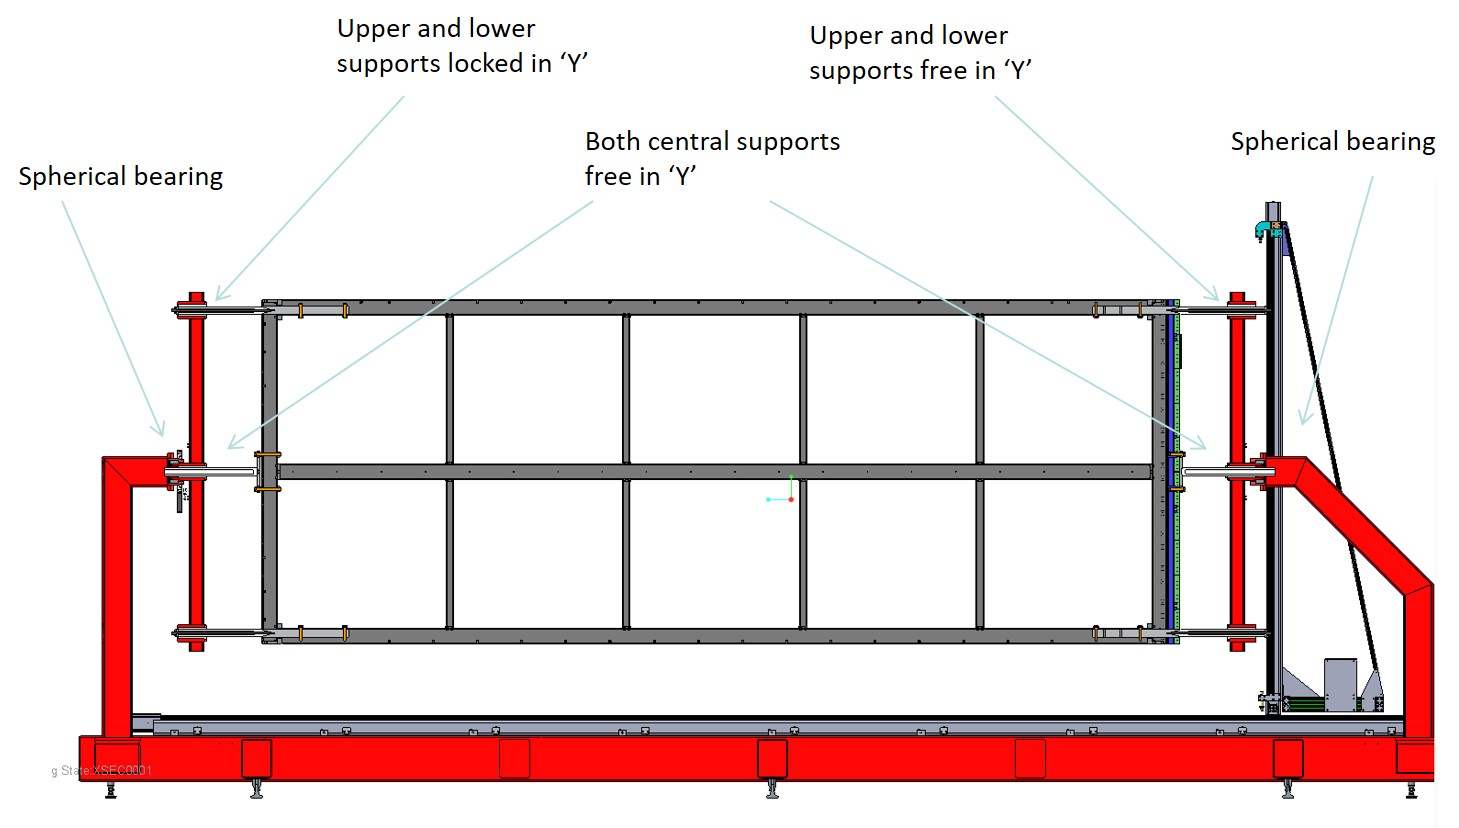
\includegraphics[width=0.95\textwidth]{Winding-machine-design-development.jpg} 
\end{dunefigure}

\item Modular mesh panels: The current approach to mesh installation is slow and cumbersome. We will improve this aspect of construction by moving toward a modular ``window screen'' design that will improve the reliability of the installed mesh (more uniform tension across the mesh), and allow much easier installation on the APA frame.

\item Epoxy process improvements: There are many epoxy application steps during the construction process. These steps require careful work that takes many hours between winding each successive wire plane. We already have concepts for improved epoxy application jigs from ProtoDUNE, and we will investigate whether epoxy pre-forms or accelerated heat curing can yield time or reliability improvements.

\item Automated soldering: Every solder joint on the 6 ProtoDUNE APAs was done by hand. We will investigate automated soldering techniques to improve process and reduce the amount of manual effort required. Commercial products exist and can be quite reliable.

\item Wire tension measurement techniques: Verifying wire tension is an important, but time consuming process during construction. The current technique utilizes a laser photodiode tool mounted on the winder to measure tension one wire at a time. This takes many hours for each wire plane. Techniques are under development at the University of Manchester to electronically measure groups of 20 or more wires at one time. This technique will provide much faster tension measurements and shorter turnaround between wire planes. 

\item Winder maintenance plan: Our current approach to winder maintenance is not well formed. As a result, winding machine problems that can be traced back to lack of routine maintenance occur from time-to-time, which shuts the production line down until a repair or maintenance is performed. We will formulate a routine and preventive maintenance plan that should minimize winder downtime.
\end{itemize}

%\todo{bring in proposed improvements table}

%%%%%%%%%%%%%%%%%%%%%%%%%%%%%%%%%%%
%\subsection{Wire Winding Machine}
%\label{sec:fdsp-apa-winding}

%\todo{Need a technical description of the current machine before going into changes}

%The design of the final wire-winding machines for DUNE far detector APAs will be based on the protoDUNE experience. The protoDUNE wire-winding machine (shown in Fig.~\ref{fig:APA-photos}) is partially automated and currently can only wire half a wire plane in a single operation. The UK and PSL engineering design staff will work to advance the design such that it is fully automated, as far as reasonably practicable.

\begin{comment}
There are several areas which can be considered for design development:
\begin{itemize}
\item Winding Head - The current winding head which carries the wire spool uses a magnetic clutch mechanism. This is manually adjusted to increase or lower the tension of the wire as it is wound around the APA. This is not an automatic process and regularly needs adjustment as the diameter of the wire on the spool reduces during the winding process. We have also found that if the mechanism is run from a `cold start' the tension changes after 10 minutes of running. Current experience of winding the ProtoDUNE wires shows that it is difficult to maintain the target tension of 5$\pm$\SI{1}{N}.

A solution to this problem is to design a winder head with active tension control. This can be achieved by replacing the magnetic clutch with a servo motor and introducing a potentiometer on a ``dancer arm'' for the feedback loop. This will only work if there are no signal losses when transferring the winding head to the compensator latching mechanism and back. The system can be driven in torque mode and will compensate for any wire spool changes and will be able to operate from a cold start. This development is well underway with tests currently being carried out. See Figure~\ref{fig:winding-head}.

\begin{dunefigure}[Exploded view of the winding machine head]{fig:winding-head}
{Exploded view of winder head with active tension control.}
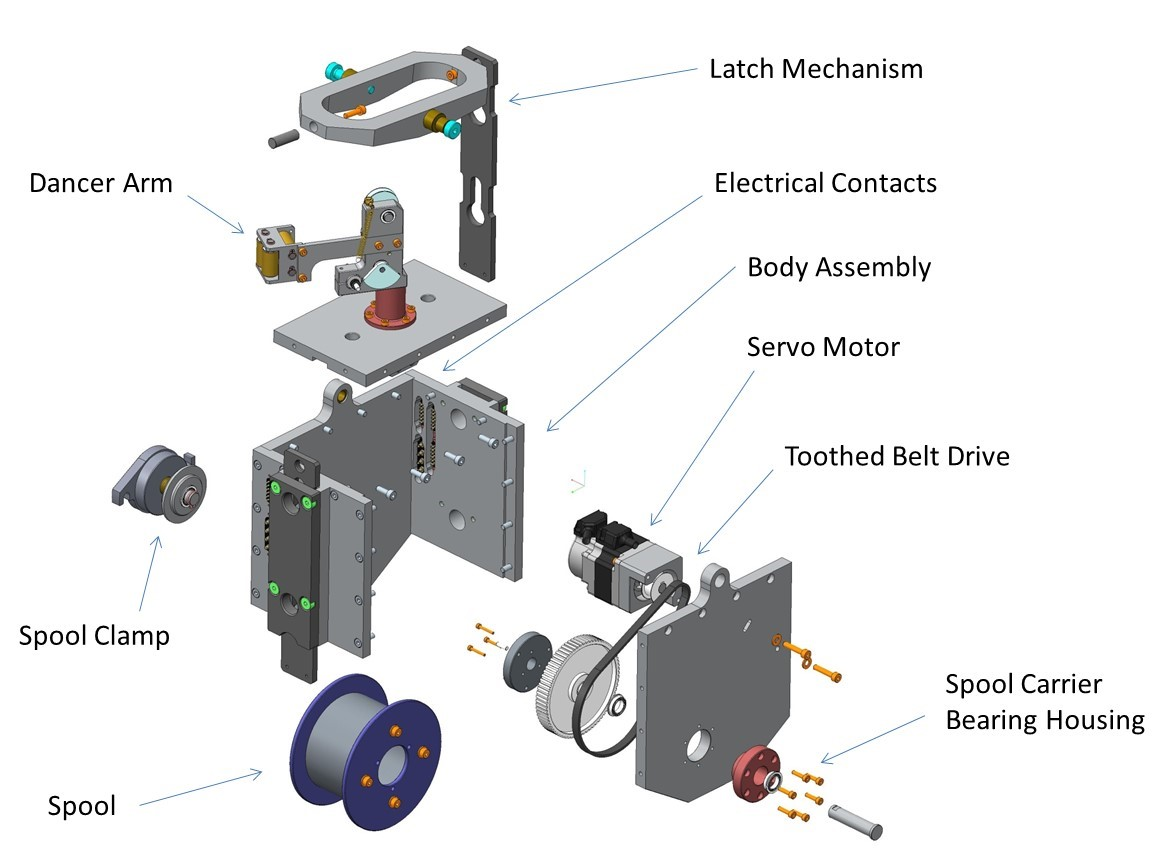
\includegraphics[width=0.7\textwidth]{Winder-head-with-active-tension-controls.jpg}
\end{dunefigure}

\item Winding Machine - To carry out the wiring operation of one full wire plane we must re-think the way in which we hold the frame in the winding machine. Holding the frame in a `flexible' manner is key to solving the current half wire winding limitations. The current method employs interface frames at the foot and head end of the machine which only allows us to wind half a wire plane. The interface frames must then be removed from the APA frame whilst it is in the process cart and flipped through 180 degs to wind the second half of the wire plane.

Design development work is in progress. The interface frames have been replaced at either end by retractable linear guided shafts. These can be withdrawn systematically to allow passing of the winding head around the frame over the full height of the frame. These shafts have conical ends and locate in shafts that are fixed to the internal frame tube to provide guided location. This design change does not alter the design of the frame, however we do not consider the riv-nuts are required and suggest that these should be omitted. The design also allows for rotation in the winding machine or the process cart for some assembly or process operations such as soldering. This is achieved using the existing features in the APA frame with the addition of a spine support at the head end.  It should also be possible to carry out board installation and gluing \& soldering in the winding machine. This eliminates the need to transfer the APA to the process cart for the whole of the production operation. This is inherently a safer production method as it cuts down the amount of handling of the APA. The development design proposal can be seen in figure??
\end{itemize}

\begin{dunefigure}[Winding Machine Dev]{fig:winding_dev}
{Winding machine design development.}
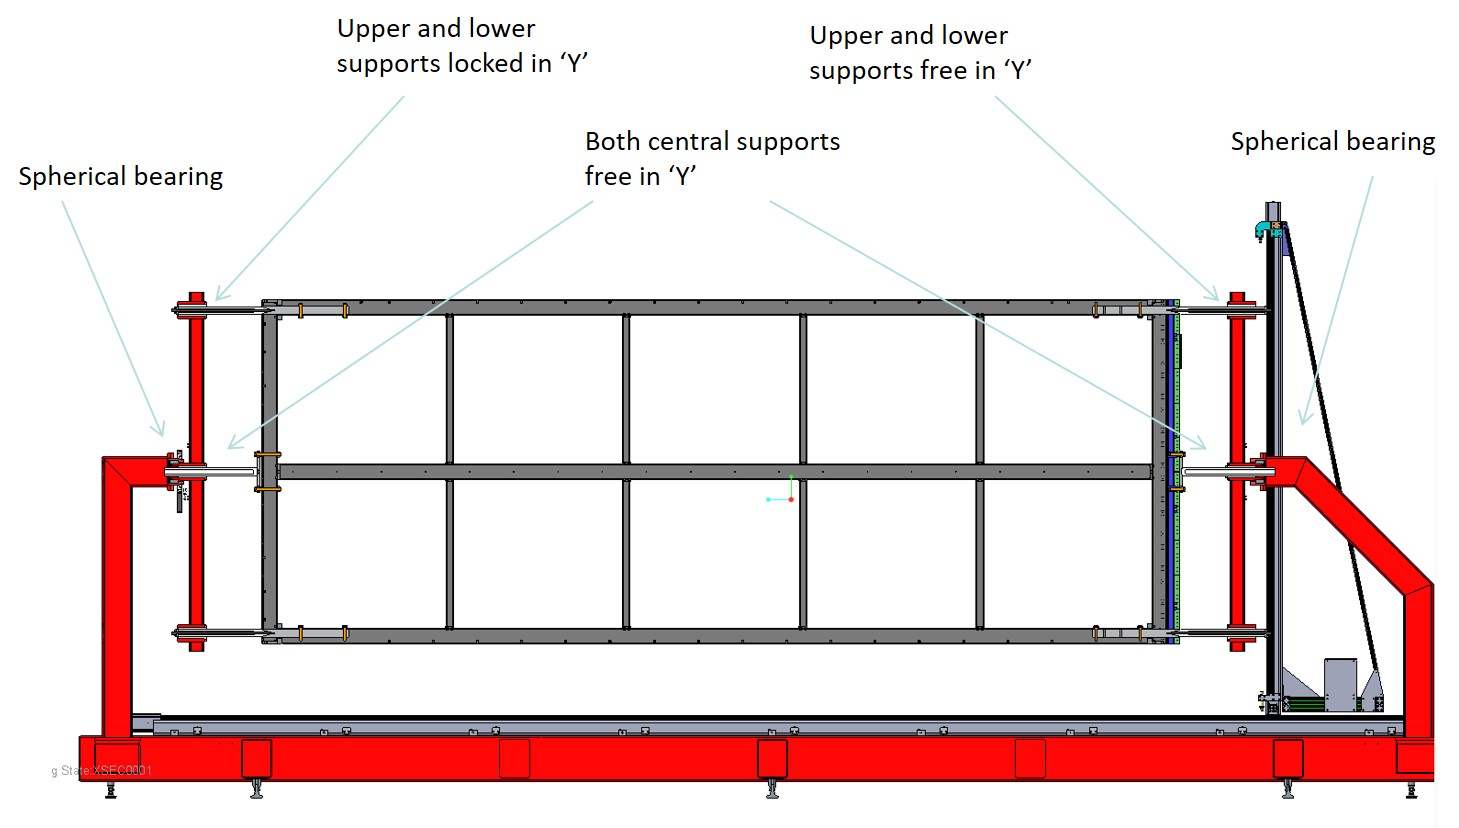
\includegraphics[width=0.8\textwidth]{Winding-machine-design-development.jpg} 
\end{dunefigure}
\end{comment}


%%%%%%%%%%%%%%%%%%%%%%%%%%%%%%%%%%%%
\subsection{Quality Assurance and Quality Control in APA Production}
\label{sec:fdsp-apa-qa}

\subsubsection{Incoming Inspections}  

Upon receipt of the rectangular hollow section steel for the frames, a selection procedure is followed to choose the sections of the steel most suited to achieving the geometrical tolerances. This procedure is documented in document PSL-TN-2013-04.  

All circuit boards that get installed to an APA are 100\% inspected for dimensional accuracy prior to being routed through various epoxy and cleaning processes as they are prepped for assembly. Inspection of boards and some other APA materials are documented in spreadsheet format, and if anomalies are found an electronic Non-Conformance report is written.  Materials that can be re-worked to become conforming are set aside from inventory and re-worked.  If the material cannot be made usable, the material is kept in a non-conforming area sequestered from usable inventory.   

\subsubsection{APA Acceptance Tests} 

The following parameters will be tested during production. Test criteria are based on requirements listed in the APA design specification and the APA requirements document. The requirements document can be found on DUNE-docdb-6416. 

\begin{itemize}
\item Frame flatness: Perform a laser survey to measure the flatness of the assembled bare frame. Three sets of data are compiled into a map that shows the amount of bow, twist, and fold in the frame. Each of these parameters is compared to an allowable amount that will not cause wire plane-to-plane spacing to be out of tolerance ($<$\SI{0.5}{mm}).  A visual file will be created for each APA from measured data. A final frame survey is completed after all electrical components have been installed, and the as-built plane-to-plane separations are measured to verify the distance between adjacent wire planes.

\item CR and G bias board testing: Acceptance tests of these boards include leakage current ($<$\SI{0.5}{nA} and continuity on each channel.  This test will be performed at room temperature. Individual components will be screened to TBD limits. ProtoDUNE was used to perform design validation on over 100 boards that were cycled and tested at LN2 temperature. No failures were seen during these tests. 

\item Mesh to frame connection: To confirm sufficient electrical contact between these two components a resistance measurement is taken in each of 20 zones of mesh bounded by the outside frame perimeter and the four cross beam ribs. This measurement is completed immediately after mesh install, prior to any winding.

\item Wire tension: Once each wire layer has been wound, the tension of each wire is measured 
%using a laser-based system. (It is hoped that an electrical system will become available in the near future.) 
Wire tensions are required to be in the range 3.5--\SI{7.5}{N} for wires longer than \SI{750}{mm} and in the range 2.0--\SI{7.5}{N} for wires shorter than \SI{750}{mm}.

\item Cleanliness: APAs are produced inside a class 100,000 clean area.  Particle counts are completed daily to verify cleanliness of the assembly area.  If counts are found outside of expected limits, measures are taken to re-clean the affected area and check with a follow-up particle count.
\end{itemize}

\subsubsection{Documentation} 

%The original procedures were created with RED TEXT that denoted to the personnel using the procedure that information or specific process data needed to be recorded into the Traveler record.  
Each APA will have a ``Traveler'' document where specific assembly information is gathered, initially by hand on a paper copy, then entered into an electronic version for longer term storage.  The Traveler database contains a detailed log of the production of each APA, including where and when the APA was built and the origin of all parts that were used in its construction. 

As assembly issues arise during the build of an APA, these are gathered in an Issue Log for each APA and separate short reports are created to provide details of what caused the occurrence, how the issue was immediately resolved, and what measures will be done in the future to ensure the specific issue has a lower risk of occurring.  %These Issues and Actions are currently being updated for US APA 2 and 3, and are currently being gathered for US APA 4.  As the documents are finished they will be uploaded to the docdb site.



%Quality Mapping Matrix A Quality Mapping Matrix has been established to ensure certain quality process steps were being performed during the assembly of an APA. We have provided an excel file with links to the associated test result files that are currently gathered during the assembly of an APA.  

%This document was placed on docdb during the summer of 2017 for test results to be reviewed as they were gathered during the build / assembly of US APA 1.  Further updates will be made to this document format to add links to all of the tests performed on US and UK APAs. 

%Incoming Inspection All circuit boards that get installed to an APA are 100\% inspected for dimensional accuracy prior to being routed through various epoxy and cleaning processes as they are prepped for assembly. Inspection of boards and some other APA materials are documented in spreadsheet format, and if anomalies are found an electronic Non-Conformance report is written.  Materials that can be re-worked to become conforming are set aside from inventory and re-worked.  If the material does become conforming, it is used on the APA.  If the material cannot be made usable, the material is kept in a non-conforming area sequestered from usable inventory.   The non-conforming reports will be reviewed and updated at the end of US APA 4 assembly to determine what materials remain that may be usable for future APA builds.

%Issue and Action Reports  As assembly issues arise during the build of an APA, these are gathered in an Issue Log for each APA and separate short reports are created to provide details of what caused the occurrence, how the issue was immediately resolved and what measures will be done in the future to ensure the specific issue has a lower risk of occurring.  These Issues and Actions are currently being updated for US APA 2 and 3, and are currently being gathered for US APA 4.  As the documents are finished they will be uploaded to the docdb site.

%\begin{dunefigure}[QC Table]{fig:qc_table}
%{placeholder until creating an actual table.}
%\includegraphics[width=0.8\textwidth]{QC-table.png} 
%\end{dunefigure}



%\fixme{Ideas from the QA plan - topics to address}
%Work processes: ensure proper training materials for and training of designers, fabricators, etc. 
%Design validation: APA has had design reviews, and is prototyped in ProtoDUNE-SP...
%Acceptance Testing of procured items? 
%Lessons learned 
%Documents and records for all these things.


